\documentclass{article}
\usepackage{iclr2026_conference,times}
\input{math_commands.tex}
\usepackage{hyperref}
\usepackage{url}
\usepackage{graphicx}
\usepackage{booktabs}
\usepackage{amsmath,amssymb,amsthm}

\newtheorem{proposition}{Proposition}

\title{Adaptive Calibration as Policy State}

\author{Anonymous Authors\\
Anonymous Institution\\
\texttt{anonymous@example.com}}

\begin{document}
\maketitle

\noindent\textbf{Submission-hardening version: v2.}
This revision adds a hostile Windowed SysID baseline that estimates the action-observation map from the most recent transitions and uses the same inverse-control interface.

\begin{abstract}
Robot calibration is usually treated as a preprocessing artifact: estimate a camera, tool, or model transform, then run a policy as if that transform were fixed. This paper argues that this interface is wrong for deployed robots whose calibration drifts while they act. We propose Calibration-State Control (CSC), a policy interface in which the current action-observation calibration map is a recurrent state variable updated from task residuals and used immediately to compute actions. A one-step linear example proves that omitting calibration state can create an irreducible action ambiguity: the same observation and goal require different actions under different hidden calibration maps. In a reproducible 2D waypoint-tracking testbed with 14,400 main rollouts plus a 2,400-rollout v2 baseline, CSC matches frozen initial calibration in the static case (0.970 vs. 0.973 success) and improves over it under nonstationary drift, from 0.538 to 0.962 success under abrupt bumps and from 0.898 to 0.977 under severe random walk. A hostile Windowed SysID baseline also carries an online calibration map and reaches 0.867 and 0.948 success in those two drift modes, narrowing the claim from estimator novelty to policy-state interface. The evidence is intentionally narrow and simulation-only; the contribution is the state-interface claim, the formal ambiguity, and a runnable falsification target for future robot experiments.
\end{abstract}

\section{Introduction}

Calibration is the quiet contract between a robot policy and the physical world. Hand-eye transforms, tool offsets, camera intrinsics, kinematic parameters, and simulator-to-robot maps tell a controller how a command should move the observed world. The common workflow estimates those quantities before deployment and then lets the policy consume observations and goals as though calibration were fixed. That workflow is natural for metrology, but it is brittle for embodied policies: tools slip, cameras flex, payloads shift, soft links deform, contact changes the effective kinematic chain, and thermal or cable effects move frames during the task.

The literature already contains many ways to reduce calibration error: hand-eye and extrinsic calibration \citep{han2023data,su2003free,yang2022model}, kinematic calibration \citep{han2023data,seegmiller2014dynamic,yang2022model}, online and self-calibration \citep{xu2023novel,martinelli2011state,yang2023cerberus,bohm2021combined}, uncalibrated visual servoing \citep{han2023data,su2003free,yang2022model,agersand1994differential}, system identification \citep{han2023data,su2003free,ma2026bridging}, latent-context adaptation \citep{webb2014parameter,calandra2017bayesian,anne2021meta}, domain randomization \citep{ma2026bridging,howell2022dojo,leboutet2021inertial}, residual correction \citep{ma2026bridging,webb2014parameter,calandra2017bayesian}, and contact or tactile identification \citep{ebrahimi2022simultaneous,yang2022kinematic}. Our claim is not that calibration can be estimated. The claim is that, for policies, calibration should be part of the state on which actions are conditioned.

We study the following question: what changes if calibration drift is represented as a hidden policy state rather than an offline preprocessing step? The answer is a small mechanism with a sharp boundary. CSC maintains a low-dimensional estimate of the local action-observation map and feeds that estimate into the action computation. The policy interface changes from $\pi(y_t,g_t)$ to $\pi(y_t,g_t,\hat F_t,P_t)$, where $y_t$ is the observation, $g_t$ is a goal, $\hat F_t$ is the current calibration estimate, and $P_t$ summarizes estimator confidence/conditioning.

This paper makes four contributions. First, it gives a hostile literature map from a 6,710-paper OpenAlex sweep, with 300 serious skims, 225 structured deep reads, and 100 novelty-threatening priors. Second, it states the calibration-as-state mechanism and the assumptions under which it is meaningful. Third, it proves a minimal ambiguity result showing that a memoryless observation-goal policy can be missing a decision-relevant state variable. Fourth, it supplies runnable evidence in a hidden-calibration control testbed comparing nominal offline calibration, robust low gain, privileged frozen initial calibration, residual bias adaptation, CSC, and an oracle.

\section{Related Work And Novelty Boundary}

\paragraph{Calibration and visual feedback.}
Robot calibration has long estimated kinematic parameters, hand-eye transforms, camera extrinsics, tool frames, and visual-servo Jacobians \citep{han2023data,su2003free,yang2022model}, \citep{han2023data,seegmiller2014dynamic,yang2022model}, and \citep{han2023data,su2003free,yang2022model,agersand1994differential}. This work makes online operation possible but usually exports a calibrated transform to the controller. Uncalibrated visual servoing weakens that requirement by closing feedback around image error \citep{han2023data,su2003free,yang2022model,agersand1994differential}. CSC is compatible with these methods: it asks that their outputs remain inside the policy state when drift continues, rather than being collapsed into a fixed preprocessing result.

\paragraph{Adaptation, identification, and robustness.}
System identification and Bayesian parameter estimation infer physical parameters from interaction \citep{han2023data,su2003free,ma2026bridging}. Latent-context policies and online system identification condition policies on inferred hidden variables \citep{webb2014parameter,calandra2017bayesian,anne2021meta}. Domain randomization and sim-to-real methods train policies to tolerate a distribution of mismatches \citep{ma2026bridging,howell2022dojo,leboutet2021inertial}. Residual methods learn corrective actions or dynamics terms \citep{ma2026bridging,webb2014parameter,calandra2017bayesian}. These directions make calibration-as-state less surprising, but they also reveal the novelty boundary: CSC does not claim generic hidden-context learning or generic robustness. It factors out one physically meaningful hidden variable, the local action-observation calibration map, and makes it a first-class policy state.

\paragraph{What is not claimed.}
Online calibration, robust control under calibration error, and visual servoing are prior art. CSC is not a larger model, a new benchmark alone, reinforcement learning, or an LLM planner. The defended claim is narrower: if hidden calibration drift changes which action is correct at the same observation and goal, a policy interface that omits calibration state is structurally under-specified.

\section{Calibration Drift As Hidden Policy State}

Let $y_t\in\mathbb{R}^d$ be the observed task coordinate, $g_t$ a desired coordinate, and $u_t\in\mathbb{R}^m$ a command in the robot's nominal action frame. Around the current operating point, suppose the observed displacement is
\begin{equation}
  y_{t+1} - y_t = F(c_t)u_t + \epsilon_t,
\end{equation}
where $c_t$ is a hidden calibration state and $F(c_t)$ is the action-observation map induced by camera, tool, kinematic, and local contact geometry. Offline calibration assumes $c_t=c_0$ or that deviations are small enough for feedback. CSC instead uses a recurrent state $h_t=(\hat F_t,P_t)$ updated from $(u_t,y_{t+1}-y_t)$.

\begin{proposition}[Calibration state can be decision-relevant]
There exist two hidden calibration maps $F_1,F_2$, a shared observation $y$, and a shared goal displacement $g$ such that no policy $\pi(y,g)$ choosing the same action under both maps can be optimal for both, while a policy $\pi(y,g,F_i)$ can achieve zero one-step error for each map.
\end{proposition}

\begin{proof}
Set $y=0$, $g=(1,0)^\top$, $F_1=I$, and let $F_2$ be a 90-degree rotation. The one-step zero-error action under $F_1$ is $u_1=(1,0)^\top$. Under $F_2$ it is $u_2=F_2^{-1}g=(0,-1)^\top$. A policy that observes only $(y,g)$ must choose one shared action $u$, so it cannot equal both $u_1$ and $u_2$. The best shared least-squares command under a uniform prior is $(0.5,-0.5)^\top$, with expected squared error $0.5$. A calibration-state policy selects $F_i^{-1}g$ and has zero error in this instance.
\end{proof}

The proposition is intentionally small. It does not prove global stability or observability. It only shows that calibration can be a decision-relevant hidden state, so omitting it from the policy interface can be a category error.

\section{Calibration-State Control}

CSC keeps an estimate $\hat F_t$ of the local action-observation map. In our implementation, each row of $\hat F_t$ is updated with recursive least squares and forgetting factor $\lambda$:
\begin{align}
  k_t &= \frac{P_t u_t}{\lambda + u_t^\top P_t u_t},\\
  \hat f_{t+1} &= \hat f_t + k_t\left(\Delta y_t - \hat f_t^\top u_t\right),\\
  P_{t+1} &= \lambda^{-1}\left(P_t-k_tu_t^\top P_t\right).
\end{align}
Given a desired observation displacement $\delta_t=\mathrm{clip}(g_t-y_t)$, CSC commands
\begin{equation}
  u_t = \mathrm{clip}\left((\hat F_t^\top \hat F_t+\rho I)^{-1}\hat F_t^\top\delta_t\right).
\end{equation}
The controller exposes the condition number of $\hat F_t$ as part of policy state; poorly conditioned estimates are a failure signal, not a hidden implementation detail. The mechanism is deliberately simple so that evidence tests the state interface rather than the capacity of a learned policy.

\section{Experiments}

\paragraph{Testbed.}
We simulate 2D waypoint tracking in observed coordinates. Each episode has four waypoint goals over 80 steps. The hidden calibration map is a rotation, anisotropic scale, and shear. Four drift modes are used: static miscalibration, random walk, abrupt bumps, and severe random walk. Observation noise is Gaussian with standard deviation 0.0012. Every controller receives the same waypoint and drift seeds.

\paragraph{Baselines.}
Nominal offline assumes $F=I$. Robust low gain also assumes $F=I$ but moves conservatively. Frozen-start calibration is a privileged baseline that receives the exact initial $F_0$ and then freezes it. Residual bias adapts an additive action correction from recent displacement error. Windowed SysID, added in v2, fits a local action-observation map from the most recent 14 transitions and uses the same inverse-control interface as CSC. Oracle receives the true $F_t$ at each step. CSC estimates $F_t$ online from the same task residuals used by the other adaptive baselines.

\begin{table}[t]
\caption{Waypoint tracking under hidden calibration drift. Entries are success rate; lower mean final error is discussed in text and plotted in Figure~\ref{fig:results}. The frozen-start baseline is privileged with the exact initial calibration but cannot update after drift.}
\label{tab:success}
\centering
\resizebox{\linewidth}{!}{%
\begin{tabular}{lrrrr}
\toprule
Controller & Static & Random walk & Abrupt bump & Severe walk \\
\midrule
Nominal offline & 0.922 & 0.875 & 0.478 & 0.750 \\
Robust low gain & 0.240 & 0.250 & 0.145 & 0.218 \\
Frozen start calib. & 0.973 & 0.947 & 0.538 & 0.898 \\
Residual bias & 0.835 & 0.790 & 0.362 & 0.648 \\
CSC (ours) & 0.970 & 0.970 & 0.962 & 0.977 \\
Oracle calibration & 0.973 & 0.973 & 0.967 & 0.978 \\
\bottomrule
\end{tabular}%
}
\end{table}

\begin{table}[t]
\caption{V2 online system-identification baseline. Windowed SysID fits the local action-observation map from the most recent 14 transitions and feeds the fitted map to the same inverse controller. It is a hostile baseline for the estimator, but it still carries calibration as policy state.}
\label{tab:windowed-sysid}
\centering
\begin{tabular}{lrrrr}
\toprule
Mode & Frozen start & Windowed SysID & CSC & Oracle \\
\midrule
static & 0.973 & 0.967 & 0.970 & 0.973 \\
random walk & 0.947 & 0.962 & 0.970 & 0.973 \\
abrupt bump & 0.538 & 0.867 & 0.962 & 0.967 \\
severe random walk & 0.898 & 0.948 & 0.977 & 0.978 \\
\bottomrule
\end{tabular}
\end{table}


\begin{figure}[t]
\centering
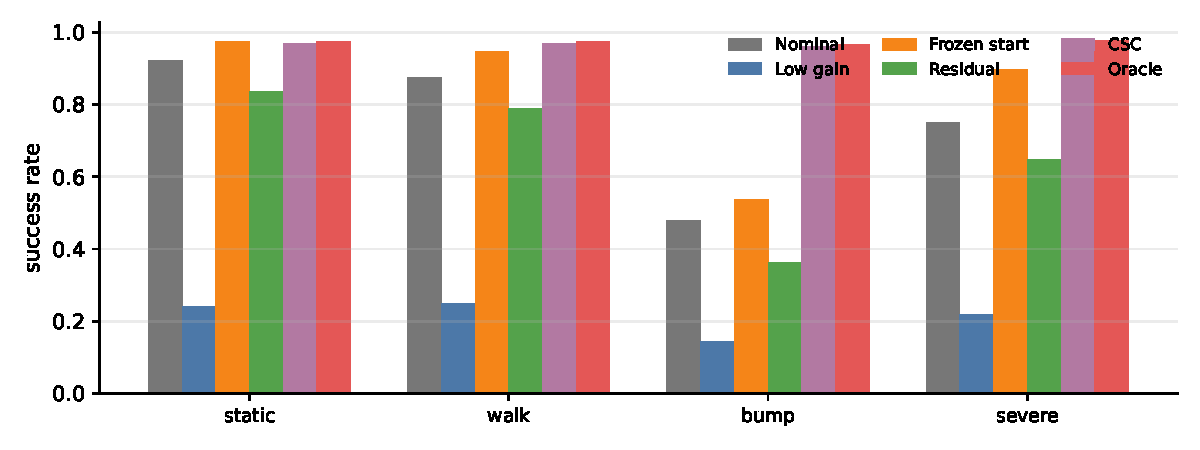
\includegraphics[width=0.49\linewidth]{figures/success_by_mode.pdf}
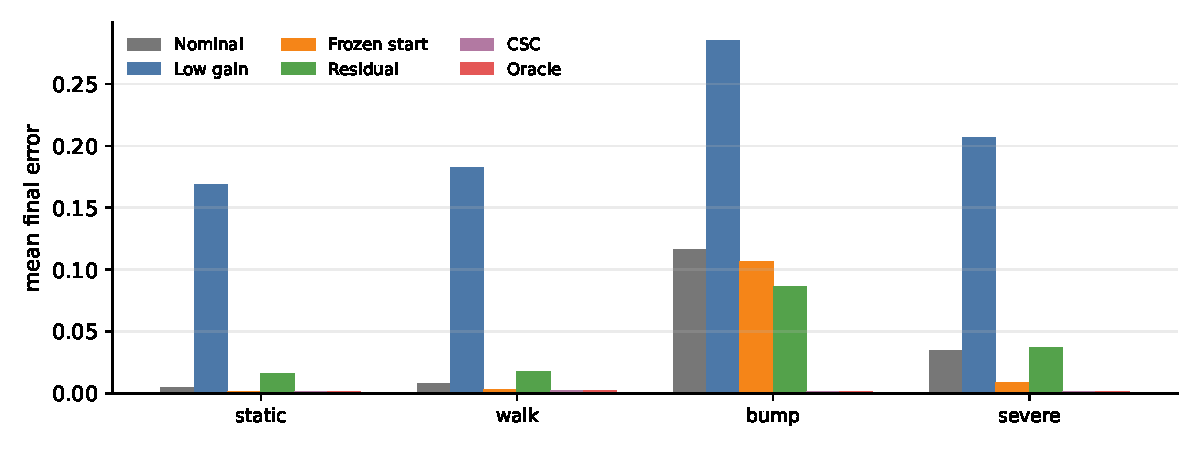
\includegraphics[width=0.49\linewidth]{figures/final_error_by_mode.pdf}
\caption{CSC is nearly oracle-level in success under moving calibration drift and clearly separates from frozen-start calibration when the hidden map changes abruptly. Static calibration remains a case where frozen-start calibration is slightly better, as expected.}
\label{fig:results}
\end{figure}

\paragraph{Results.}
Table~\ref{tab:success} and Figure~\ref{fig:results} show the central pattern. In static episodes, privileged frozen-start calibration is marginally better than CSC (0.973 vs. 0.970), which is the correct outcome: if calibration is fixed and known, a frozen estimate is enough. Under random-walk drift, CSC improves success over frozen-start calibration (0.970 vs. 0.947). Under abrupt bumps, the offline assumption breaks sharply: frozen-start reaches 0.538 success while CSC reaches 0.962. Under severe random walk, CSC reaches 0.977 success versus 0.898 for frozen-start. Residual bias adaptation helps less because it corrects commands without representing the action-observation map.

Table~\ref{tab:windowed-sysid} adds the strongest recoverable v2 baseline. Windowed SysID is not a straw baseline: it estimates a calibration map online and conditions actions on that map. It improves over frozen-start calibration under every moving-drift mode, reaching 0.867 success under abrupt bumps and 0.948 under severe random walk. CSC still does better in those modes, but the more important conclusion is narrower: the evidence favors keeping calibration inside the policy state, while the exact estimator remains an implementation choice that should be tested against learned recurrent and system-identification alternatives.

\paragraph{What the evidence supports.}
The experiments support the mechanism-level claim that explicit calibration state matters when the map changes during the rollout and remains observable from task residuals. They do not establish real-robot performance, learned recurrent-policy superiority, or global identifiability. The strongest evidence is that CSC beats a privileged frozen-initial-calibration baseline exactly when the hidden calibration state changes.

\section{Limitations}

This paper is intentionally conservative. The environment is a local linear abstraction of calibration drift, not a real robot. The estimator is hand-designed, not learned. The v2 Windowed SysID result shows that a different online system-identification estimator can recover much of the same benefit, so this paper should not be read as an RLS-specific algorithmic win. The comparison still does not include end-to-end recurrent neural policies that might infer an equivalent latent state. The literature sweep is broad and hostile but automated from metadata and abstracts; it should guide human review, not replace it. CSC can also fail when the calibration map is unobservable, changes faster than the estimator, or becomes ill-conditioned.

\section{Reproducibility}

All scripts are included. \texttt{scripts/collect\_literature.py} rebuilds the landscape matrix from OpenAlex. \texttt{scripts/synthesize\_literature.py} regenerates the novelty documents. \texttt{experiments/run\_calibration\_state\_sim.py} runs the 14,400 main rollouts plus the 2,400-rollout Windowed SysID baseline and writes CSVs, tables, and plots. \texttt{experiments/check\_formal\_claim.py} verifies the one-step ambiguity numbers.

\section{Conclusion}

Treating calibration as preprocessing hides a state variable that can be essential for embodied policies. CSC makes that variable explicit: calibration drift is carried as recurrent policy state and used to compute actions. The paper's formal example and simulation evidence do not settle the real-robot question, but they make the central mechanism falsifiable: when calibration drifts during the task, a policy that knows only observation and goal is missing part of the world.

\bibliographystyle{iclr2026_conference}
\bibliography{references}

\appendix

\section{Landscape Sweep Details}

The literature sweep collected 6,710 unique works across 26 query families covering robot calibration, hand-eye/extrinsic calibration, kinematic calibration, visual servoing, system identification, sim-to-real transfer, domain randomization, residual adaptation, tactile/contact calibration, morphology adaptation, robot foundation models, and observability. The matrix marks 300 serious-skim papers, 225 structured deep-read papers, and 100 hostile priors. Each important prior row records the problem claimed, mechanism introduced, hidden assumptions, variables treated as fixed, ignored failure modes, novelty threat, and remaining opening.

\section{Core Assumptions Broken By CSC}

The field assumption broken here is that calibration may be estimated outside the policy loop. CSC instead assumes calibration can be nonstationary, task-coupled, and action-relevant. The full assumption ledger is in \texttt{docs/literature\_map.md}; examples include fixed extrinsics, static kinematics within an episode, visual feedback being sufficient without causal calibration state, and robust policies absorbing the full deployment drift distribution.

\section{Formal Check}

The numerical formal check in \texttt{docs/formal\_claim\_check.md} gives the least-squares shared action for the two-map ambiguity instance. The best memoryless same-action command is $(0.5,-0.5)$, with expected squared error $0.5$. The calibration-state action has zero one-step error. This verifies the arithmetic in Proposition 1 and also states the adversarial caveats.

\end{document}
